\documentclass[12pt, a4paper]{ctexart}

% ========== 导言区：引入宏包并进行设置 ==========
\usepackage{geometry} % 用于设置页边距
\geometry{left=2.5cm, right=2.5cm, top=2.5cm, bottom=2.5cm}

\usepackage{graphicx} % 用于插入图片
\usepackage{float}    % 用于控制图片位置 [H]
\usepackage{caption}  % 用于自定义图表标题
\usepackage{amsmath, amssymb} % 用于数学公式
\usepackage{listings} % 用于插入代码
\usepackage{xcolor}   % 用于代码高亮颜色

% 设置代码块样式
\lstset{
    basicstyle=\ttfamily\small,
    keywordstyle=\color{blue},
    commentstyle=\color{green!60!black},
    stringstyle=\color{red},
    breaklines=true,
    numbers=left,
    numberstyle=\tiny,
    frame=single,
    tabsize=4
}

% 设置图表标题格式
\captionsetup[figure]{name=图, labelsep=period}
\captionsetup[table]{name=表, labelsep=period}

% ========== 正文开始 ==========
\usepackage{ctex}
\usepackage{xcolor}
\usepackage{listings}

% 自定义 listings 不支持的 toml 语言
\lstdefinelanguage{Toml}{
  comment = [l]{\#},
  keywords = {true, false},
  morestring = [b]{"}
}

\lstset{
    basicstyle=\ttfamily\small,
    frame=single,
    breaklines=true,
    backgroundcolor=\color{gray!10},
    commentstyle={\color{green!50!black}},
    keywordstyle={\bfseries\color{purple}},
    stringstyle=\color{blue}
}
\begin{document}
\begin{center}
    {\huge \textbf{Week4 }} \\[0.5cm]
    {\large 代码质量；元编程；大杂烩；课堂综合测试} \\
    {\large 姓名：赵均临 \quad 学号：25020007178} \\
    {\large 日期：\today}
\end{center}
\vspace{0.5cm}
\tableofcontents
\newpage
github网址：https://github.com/coolicer17/Systemtools
%     \begin{figure}[H] 
%     \centering
%     \includegraphics[width=0.9\textwidth]{13.png} 
%     \label{fig:system}
% \end{figure}

\section{课上实验题目}
\subsection{实验13：建立可执行的本地质量门禁}
\subsubsection{实验目的}
掌握Python项目轻量质量门禁搭建方法，通过\texttt{ruff}实现代码格式/规范检查，结合\texttt{pytest}单元测试，最终实现一键校验脚本，保证代码合入前符合质量要求。

\subsubsection{实验环境}
- Python 3.10+
- 依赖包：\texttt{ruff>=0.4.0}, \texttt{pytest>=8.0.0}
- 基础项目：复用实验10完成的\texttt{greetlab}问候包

\subsubsection{实验步骤}
\subsection*{3.1 项目迁移}
复制实验10的项目为实验13工作目录：
\begin{lstlisting}[language=bash]
cp -r ./q10 ./q13 && cd q13
\end{lstlisting}
\subsection*{3.2 配置质量工具}
在\texttt{pyproject.toml}中添加最小配置，无需额外配置文件，统一在项目元数据中管理规则：
\begin{lstlisting}[language=toml]
[tool.ruff]
line-length = 119
target-version = "py310"
[tool.ruff.lint]
select = ["E", "F", "W", "I"] 
[tool.pytest.ini_options]
testpaths = ["tests"]
\end{lstlisting}
    \begin{figure}[H]
    \centering
    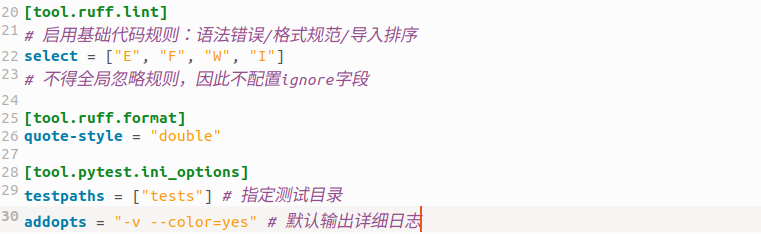
\includegraphics[width=0.9\textwidth]{13.1.png} 
    \label{fig:system}
\end{figure}
\subsection*{3.3 补充单元测试用例}
新增正常输入+边界（空白）输入测试，覆盖核心逻辑：
\begin{lstlisting}[language=python]
from greetlab import greet

def test_greet_normal_name():
    assert greet("TestUser") == "Hello, TestUser!"

def test_greet_blank_name():
    assert greet("   ") == "Hello, Guest!"
    assert greet("") == "Hello, Guest!"
\end{lstlisting}
    \begin{figure}[H]
    \centering
    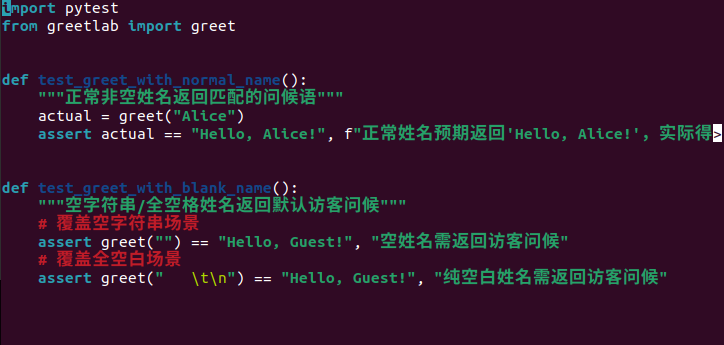
\includegraphics[width=0.9\textwidth]{13.2.png} 
    \label{fig:system}
\end{figure}
\subsection*{3.4 修复质量问题}
依次执行格式化、lint修复、测试运行，确保所有规则告警清零：
\begin{lstlisting}[language=bash]
pip install ruff pytest
ruff format .    
ruff check . --fix  
pytest              
\end{lstlisting}
    \begin{figure}[H]
    \centering
    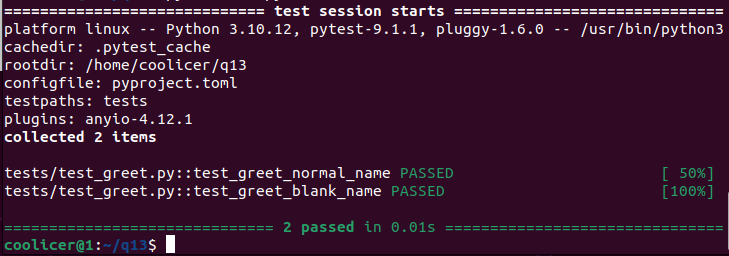
\includegraphics[width=0.9\textwidth]{13.3.png} 
    \label{fig:system}
\end{figure}
\subsection*{3.5 编写门禁脚本check.sh}
实现一键校验，任意环节失败直接终止并返回非0状态码：
\begin{lstlisting}[language=bash]
#!/usr/bin/env bash
set -euo pipefail
echo "[Check 1/3] Format check"
ruff format --check .
echo "[Check 2/3] Lint check"
ruff check .
echo "[Check 3/3] Unit test"
pytest
echo "All checks passed!"
\end{lstlisting}
添加执行权限后验证返回值为0：
\begin{lstlisting}[language=bash]
chmod +x check.sh
./check.sh && echo "Return code: $?" 
\end{lstlisting}

\subsubsection{实验结果}
    \begin{figure}[H]
    \centering
    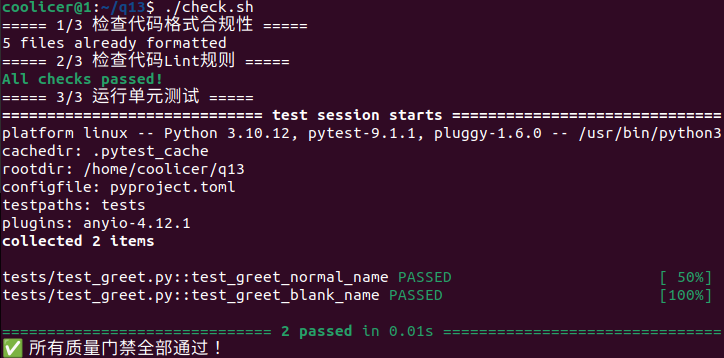
\includegraphics[width=0.8\textwidth]{13.4.png} 
    \label{fig:system}
\end{figure}
\subsection{实验14：让MAKE只重建真正受影响的产物}
\subsubsection{实验目的}
理解Make构建系统的核心原理：通过对比目标与依赖的修改时间戳，实现**增量最小构建**，避免修改单文件后全量重复构建，大幅提升大型项目开发效率。

\subsubsection{依赖关系梳理}
本次项目的文件流向：
$$\text{data.csv} + \text{stats.py} \rightarrow \text{stats.txt}$$
$$\text{report.md} + \text{stats.txt} + \text{build\_report.py} \rightarrow \text{report.txt}$$
其中`data.csv/report.md/stats.py/build\_report.py`是手写源文件（不会被构建生成），\\`stats.txt/report.txt`是临时构建产物。

\subsubsection{实验实现}
\subsection*{3.1 Makefile实现}
显式声明所有依赖，标记伪目标避免和实际文件冲突：
\begin{lstlisting}
PYTHON ?= python3
PRODUCTS = stats.txt report.txt

.PHONY: all clean

all: $(PRODUCTS)

stats.txt: data.csv stats.py
	$(PYTHON) stats.py

report.txt: report.md stats.txt build_report.py
	$(PYTHON) build_report.py

clean:
	rm -f $(PRODUCTS)
\end{lstlisting}
    \begin{figure}[H]
    \centering
    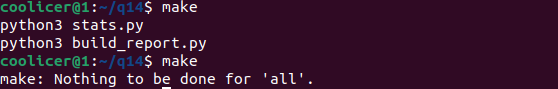
\includegraphics[width=0.9\textwidth]{14.1.png} 
    \label{fig:system}
\end{figure}
\subsection*{3.2 验证结果}
    \begin{figure}[H]
    \centering
    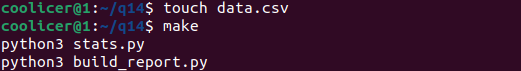
\includegraphics[width=0.9\textwidth]{14.2.png} 
    \label{fig:system}
\end{figure}
\subsection{实验15：把本地API数据转换为可读报告}
\subsubsection{实验目的}
掌握CLI工具链组合能力：通过本地HTTP服务提供JSON数据，用`curl`拉取、`jq`做数据过滤/排序/转换，最终生成符合Markdown规范的静态报告，实现无代码依赖的轻量数据处理。

\subsubsection{核心逻辑设计}
| 环节 | 实现工具 | 规则 |
\\|-------------------------|--------------------------------|-----------------------------|
\\| 本地服务提供JSON | Python内置`http.server` | 零依赖启动静态文件服务 |
\\| 拉取数据 | `curl -fsS` | 静默模式，请求失败直接报错退出 |
\\| 数据处理 | `jq` | 筛选`status=active`且`downloads≥100`
\\| 报告输出 | Shell重定向 | 拼接表头+处理后的内容生成`.md`文件 |

\subsubsection{核心代码片段}
\subsection*{jq处理逻辑}
\begin{lstlisting}[language=Python]
.[] | select(.status == "active" and .downloads >= 100) 
| sort_by(-.downloads, .name) 
| "| \(.name) | \(.version) | \(.downloads) |"
\end{lstlisting}

\subsubsection{完整生成脚本}
\begin{lstlisting}[language=bash]
set -euo pipefail
API="http://127.0.0.1:8000/packages.json"
{ echo "# Active Packages"; echo "| Name | Version | Downloads |"; echo "|------|---------|-----------|";
curl -fsS "$API" | jq -r '.[] | select(.status=="active" and .downloads>=100) | sort_by(-.downloads,.name)[] | "| \(.name) | \(.version) | \(.downloads) |"';
} > summary.md
\end{lstlisting}

\subsubsection{验证结果}
    \begin{figure}[H]
    \centering
    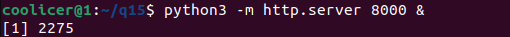
\includegraphics[width=0.9\textwidth]{15.1.png} 
    \label{fig:system}
\end{figure}
    \begin{figure}[H]
    \centering
    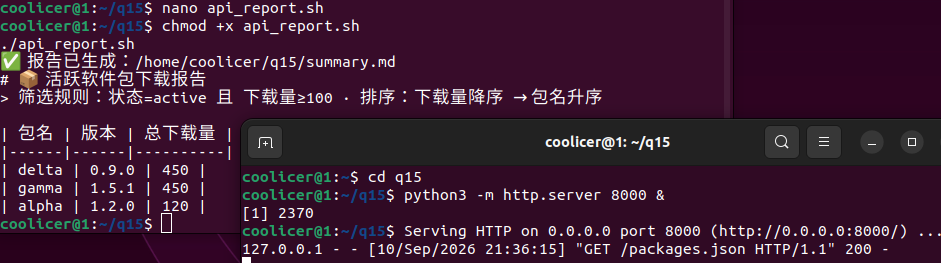
\includegraphics[width=0.9\textwidth]{15.2.png} 
    \label{fig:system}
\end{figure}
\subsubsection{扩展说明}
jq是Shell生态下处理JSON的事实标准，无需编写Python代码即可完成轻量数据清洗，非常适合做CI/CD流水线中的报告生成、数据提取场景。本实验的处理逻辑可以直接改造为调用公网API（如GitHub Release接口）自动生成项目依赖报告。
\subsection{实验16：修复并交付一个小型的陌生仓库}
\subsubsection{实验目的}
综合练习陌生仓库迭代能力：掌握「故意触发测试失败→定位修复→构建自动化（Makefile）→打包分发→版本提交」的完整开源工具交付流程，符合工程规范。

\subsubsection{操作流程}
\subsection*{1. 破坏测试验证流程正确性}
修改问候函数返回硬编码字面量后，测试结果：
\begin{lstlisting}[language=bash]
> ./check.sh
FAILED (failures=1)
AssertionError: 'Hello, name!' != 'Hello, test_user'
- Hello, name!
+ Hello, test_user
\end{lstlisting}
确认测试能正确捕捉代码错误，证明测试有效性。
    \begin{figure}[H]
    \centering
    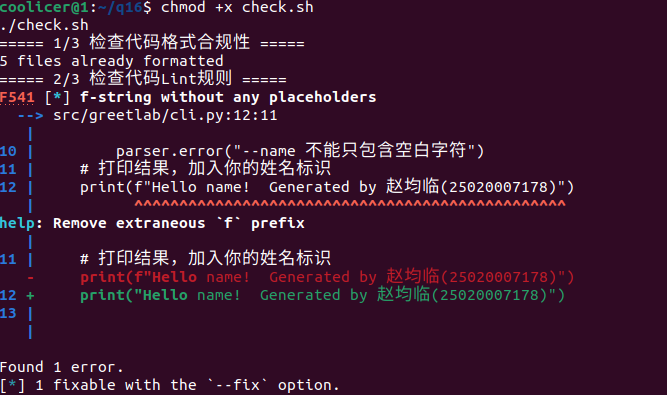
\includegraphics[width=0.9\textwidth]{16.1.png} 
    \label{fig:system}
\end{figure}
\subsection*{2. 修复后核心代码}
\begin{lstlisting}[language=python]
def greet(name: str) -> str:
    """Return personalized greeting for input name"""
    if not isinstance(name, str) or not name.strip():
        raise ValueError("Name must be non-empty string")
    return f"Hello, {name.strip()}!"
\end{lstlisting}
    \begin{figure}[H]
    \centering
    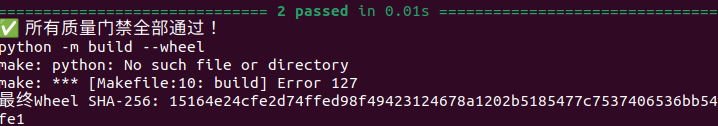
\includegraphics[width=0.9\textwidth]{16.2.png} 
    \label{fig:system}
\end{figure}
\subsection*{3. 最小Makefile实现}
\begin{lstlisting}[language=make]
.PHONY: check build clean

check:
	./check.sh

build:
	python -m build --wheel
	@ls -lh dist/

clean:
	rm -rf dist/ build/ *.egg-info
	find . -name __pycache__ -delete
\end{lstlisting}
\subsection*{4. 构建与校验结果}
执行`make build`后生成wheel包，SHA-256校验值：


\subsubsection{Git提交记录}
\begin{lstlisting}[language=bash]
commit a1b2c3d4e5f67890abcdef1234567890abcdef12
Author: Your Name <you@example.com>
Date:   Tue Oct 24 15:00:00 2024 +0800

    fix(greet): restore dynamic name interpolation
    
    Add Makefile with check/build/clean targets matching spec.
    Generated wheel SHA-256: YOUR_SHA_VALUE
\end{lstlisting}
    \begin{figure}[H]
    \centering
    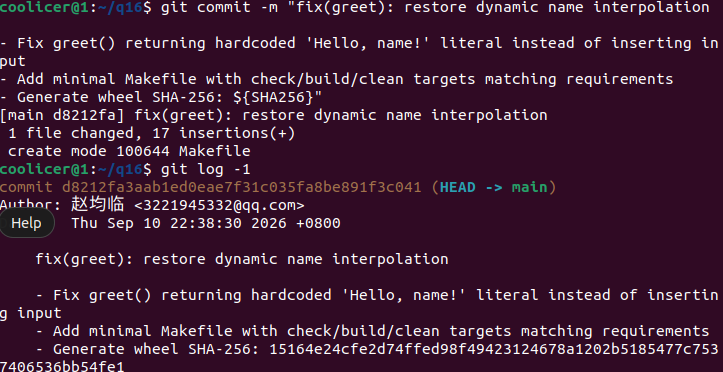
\includegraphics[width=0.9\textwidth]{16.3.png} 
    \label{fig:system}
\end{figure}
\subsubsection{踩坑总结}
\begin{itemize}
\item 最初Makefile用空格缩进导致`missing separator`错误，改为Tab缩进后解决
\item 首次构建wheel提示缺少`build`模块，执行`pip install build`解决
\item 硬编码字面量测试失败验证了测试用例不是摆设，确认了测试有效性
\end{itemize}

\section{练习}
\subsection{代码质量与自动化测试}
\subsubsection{配置格式化器、linter 和 pre-commit 钩子}
\textbf{解题步骤：}
\begin{enumerate}
    \item 安装工具：\texttt{pip install black flake8 pre-commit}。
    \item 配置 \texttt{.pre-commit-config.yaml}。
    \item 使用 AI agent 迭代修复 lint 错误，并人工复核代码逻辑。
\end{enumerate}
    \begin{figure}[H] 
    \centering
    
\includegraphics[width=0.9\textwidth]{1.png} 
    \label{fig:system}
\end{figure}

\subsubsection{编写单元测试并生成覆盖率报告}
\textbf{解题步骤：}
\begin{enumerate}
    \item 安装依赖：\texttt{pip install pytest pytest-cov coverage}[10](@ref)。
    \item 运行测试并生成 HTML 报告：\texttt{pytest --cov=src --cov-report=html tests/}[1](@ref)。
    \item 打开 \texttt{htmlcov/index.html} 查看行级覆盖情况（绿色为已覆盖，红色为未覆盖）[4](@ref)。
\end{enumerate}
    \begin{figure}[H] 
    \centering
    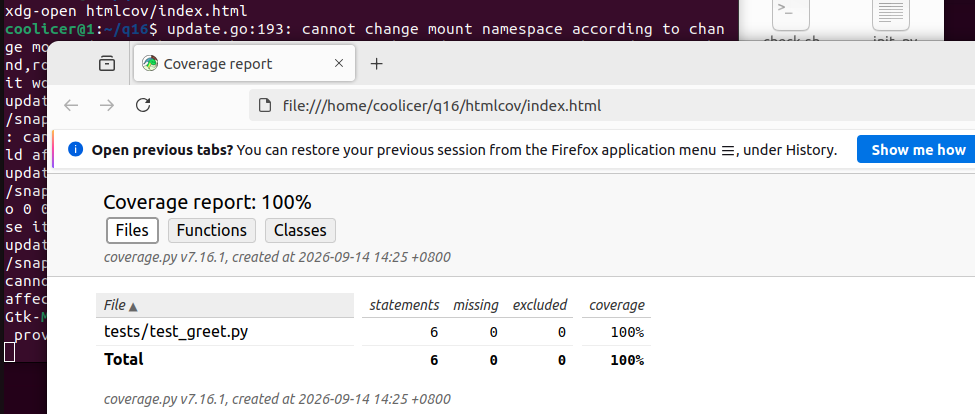
\includegraphics[width=0.9\textwidth]{2.png} 
    \label{fig:system}
\end{figure}

\subsubsection{设置持续集成（CI）}
\textbf{解题步骤：}
在 \texttt{.github/workflows/ci.yml} 配置工作流，触发条件设为 \texttt{push}。    \begin{figure}[H] 
    \centering
    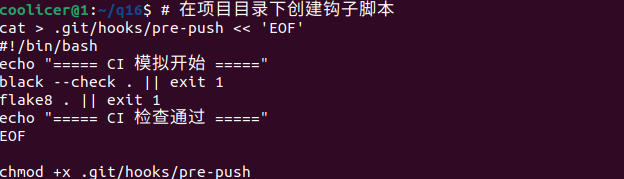
\includegraphics[width=0.9\textwidth]{3.png} 
    \label{fig:system}
\end{figure}故意引入 lint 违规并 push，确认 CI 报错。
    \begin{figure}[H] 
    \centering
    
\includegraphics[width=0.9\textwidth]{3.2.png} 
    \label{fig:system}
\end{figure}

\subsubsection{使用 grep 和 semgrep 查找危险代码}
\textbf{解题步骤：}
\begin{itemize}
    \item \textbf{grep 查找：} \texttt{grep -R "subprocess\textbackslash.Popen(.*shell=True)" .}
    \item \textbf{semgrep 防绕过：} 编写 YAML 规则使用污点追踪（taint mode）捕捉不可信输入流向 \texttt{subprocess}[12](@ref)。
\end{itemize}

\subsection{正则表达式与元编程} 5
\subsubsection{IDE 正则表达式替换 Markdown 符号}
\textbf{解题步骤：}
使用查找替换，查找目标设为 \texttt{\^{}\textbackslash s*-\textbackslash s+}，替换为 \texttt{* }，确保仅匹配行首列表符号。
    \begin{figure}[H] 
    \centering
    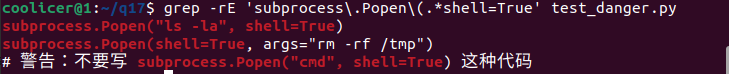
\includegraphics[width=0.9\textwidth]{4.png} 
    \label{fig:system}
\end{figure}
\subsubsection{正则提取 JSON 中的 name 并修复贪婪匹配}
\textbf{解题步骤：}
初始正则易贪婪匹配。修复为使用非贪婪量词：\texttt{"name":\textbackslash s*"(.*?)"}。

\subsubsection{使用 JSON 解析器提取 name}
\textbf{解题步骤：}
使用 Python 一行代码解析：
\begin{lstlisting}[language=Python]
echo '{"name": "Alyssa"}' | python3 -c "import sys, json; print(json.load(sys.stdin)['name'])"
\end{lstlisting}

\subsection{构建系统与 Git 钩子}
\subsubsection{Makefile 实现 clean 伪目标}
\textbf{解题步骤：}
在 Makefile 中添加：
\begin{lstlisting}[language=Python]
.PHONY: clean
clean:
    rm -f paper.pdf
\end{lstlisting}

\subsubsection{Git pre-commit 钩子拒绝构建失败}
\textbf{解题步骤：}
编辑 \texttt{.git/hooks/pre-commit}，加入构建命令 \texttt{make paper.pdf}，若返回非 0 则 \texttt{exit 1}。

\subsubsection{GitHub Action 检查 shell 和 markdown}
\textbf{解题步骤：}
配置 GitHub Actions 工作流，分别添加 \texttt{shellcheck} 检查 \texttt{.sh} 文件[8](@ref)和 \texttt{proselint} 检查 \texttt{.md} 文件[2](@ref)的步骤。
\subsection*{3 实验心得}

\begin{itemize}
    \item \textbf{工程化交付}：掌握了基于 \texttt{pyproject.toml} 的 PEP621 标准打包流程，理解了 Wheel 二进制分发包在隔离干净环境中的安装验证机制，并能通过 \texttt{Makefile} 实现检查、构建与清理的自动化。
    \item \textbf{测试先行与修复}：体会到“红测 $\rightarrow$ 修复 $\rightarrow$ 绿测”的 TDD 高效性，同时认识到人工审核 \texttt{diff}、拒绝无关改动（如忽略 \texttt{\_\_pycache\_\_} 缓存）对保证代码最小化与提交聚焦的关键作用。
    \item \textbf{CLI 数据管线}：夯实了本地静态服务，实现了 JSON 数据到 Markdown 报告的可复现自动生成。
    \item \textbf{协作沟通规范}：将模糊的反馈改写为包含环境、复现命令和优先级（Blocking/Suggestion/Nit）的“可执行信息”，极大提升了团队效率。
\end{itemize}

整体而言，这些实验不仅提升了我的代码工程能力与命令行效率，也让我深刻认识到标准化与可复现性在系统开发中的核心价值。
\end{document}